% Figure: the echo of A-contrast-memory-spherical-v1 on one seam: write, phase, reverse write.
\begin{tikzpicture}[x=1cm,y=1cm,
  cms wire/.style={black!70, line width=0.6pt},
  cms mem/.style={black!70, line width=0.6pt, dash pattern=on 2.5pt off 1.5pt},
  cms gate/.style={draw=black, fill=black!6, rounded corners=1.5pt, line width=0.6pt,
    align=center, font=\footnotesize, inner sep=3pt},
  cms note/.style={font=\scriptsize, text=black!80, align=center, inner sep=1pt}]
% wires
\draw[cms wire] (0,1.7)--(11.7,1.7);
\draw[cms wire] (0,0.8)--(11.7,0.8);
\draw[cms mem] (0,-0.6)--(11.7,-0.6);
\node[anchor=east, font=\footnotesize] at (-0.1,1.7) {port $a$, load $n_a$};
\node[anchor=east, font=\footnotesize] at (-0.1,0.8) {port $b$, load $n_b$};
\node[anchor=east, font=\footnotesize, align=right] at (-0.1,-0.6) {private\\[-1pt]seam memory};
% gates
\node[cms gate, minimum width=1.5cm, minimum height=3.1cm] (W) at (2.2,0.55) {write\\$W$};
\node[cms gate, minimum width=2.4cm, minimum height=0.95cm] (Ph) at (5.85,-0.6)
  {phase\\$e^{-i\tau M_\kappa}$};
\node[cms gate, minimum width=1.5cm, minimum height=3.1cm] (Wd) at (9.5,0.55) {reverse\\write $W^{*}$};
% contents of the memory along the wire
\node[cms note, anchor=south] at (0.7,-0.55) {blank};
\node[cms note, anchor=south] at (3.8,-0.55) {$(c,d)$};
\node[cms note, anchor=south] at (7.9,-0.55) {$(c,\pm d)$};
\node[cms note, anchor=south] at (11.0,-0.55) {blank};
% contents of the ports between the two writes
\node[cms note, fill=white, inner sep=2pt] at (5.85,1.25) {output $y_c(n_a,n_b)$ of the native seam event};
\node[cms note, anchor=north] at (5.85,-1.25)
  {$M_\kappa=\tfrac12(I-R)+\kappa D^{2}$: $R$ reverses the contrast, $D^{2}$ charges its square};
\node[font=\footnotesize, anchor=north] at (5.85,-1.85)
  {on the two loads the three steps are
   $\exp\bigl(-i\tau\bigl[\tfrac12(I-\mathrm{SWAP})+\kappa\,(n_a-n_b)^{2}\bigr]\bigr)$};
\end{tikzpicture}
